% \begin{center}
%     \captionof{figure}{Bias for DGM 1 in Within-Person and Contextual Effect for Different Estimation Approaches}
%     \begin{subfigure}{0.49\linewidth}
%         \centering
%         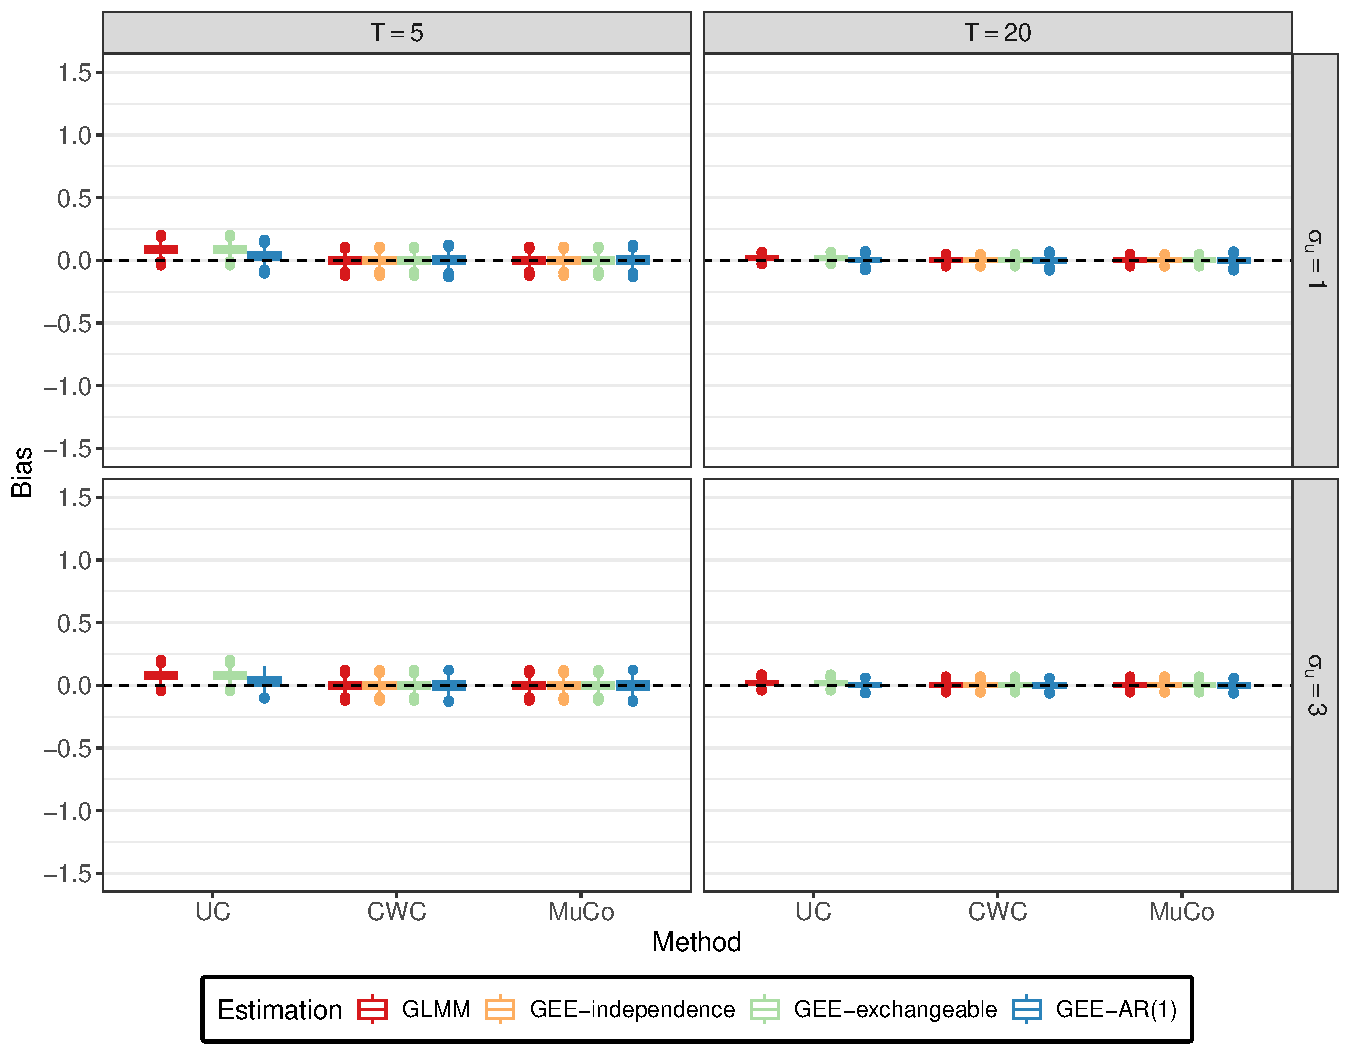
\includegraphics[width=\linewidth, keepaspectratio]{Figures/pred_continuous_out_continuous_bias_plot_T_total-vs-sd.u0_within.pdf}
%         \caption{Within-Person Effect}\label{fig:dgm1-within}
%     \end{subfigure}
%     \hfill
%     \begin{subfigure}{0.49\linewidth}
%         \centering
%         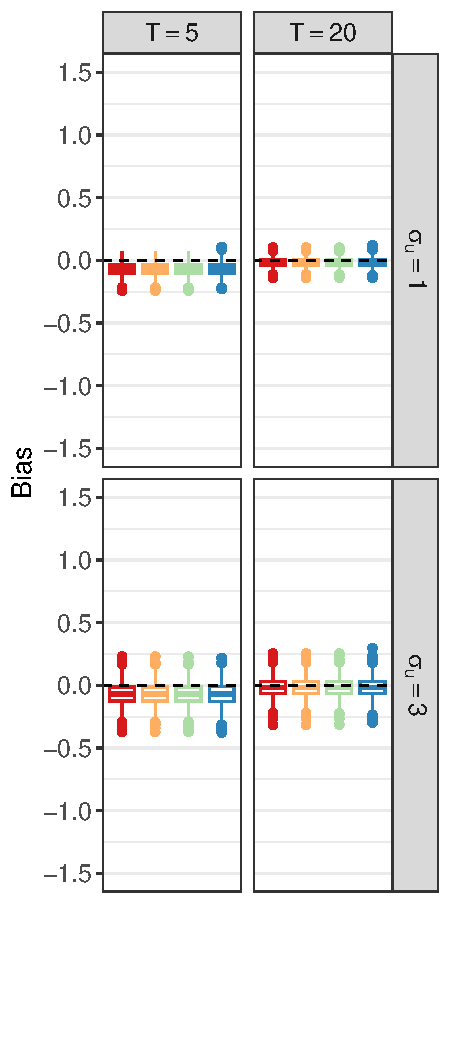
\includegraphics[height=6, keepaspectratio]{Figures/pred_continuous_out_continuous_bias_plot_T_total-vs-sd.u0_contextual.pdf}
%         \caption{Contextual Effect (Method 3)}\label{fig:dgm1-contextual}
%     \end{subfigure}
%     \label{fig:dgm1}
%     % \begin{figurenote}
%     %     \ldots
%     % \end{figurenote}
% \end{center}

\begin{center}
    \captionof{figure}{Bias for DGM 1 in Within-Person and Contextual Effect for Different Estimation Approaches}
     \hspace*{-1.5cm}
    \begin{subfigure}{0.80\linewidth}  % Set width proportionally for the first figure
        \centering
        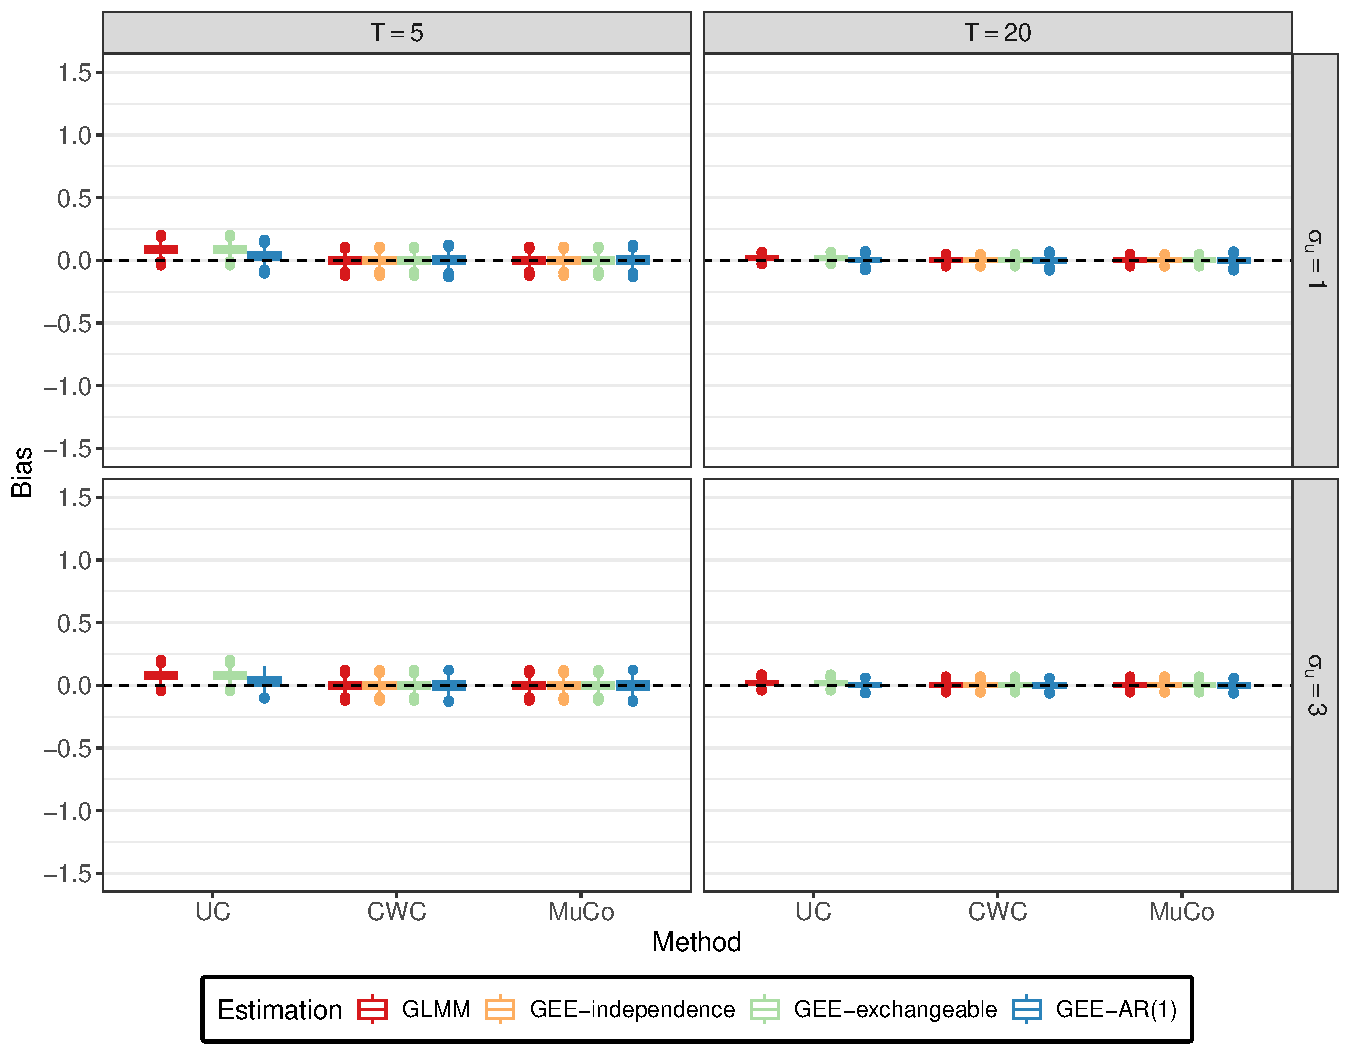
\includegraphics[height=10.6cm, keepaspectratio]{Figures/pred_continuous_out_continuous_bias_plot_T_total-vs-sd.u0_within.pdf}
        \caption{Within-Person Effect $\beta_1$}\label{fig:dgm1-within}
    \end{subfigure}
    \hfill
    \begin{subfigure}{0.25\linewidth}  % Set width proportionally for the second figure
        \centering
        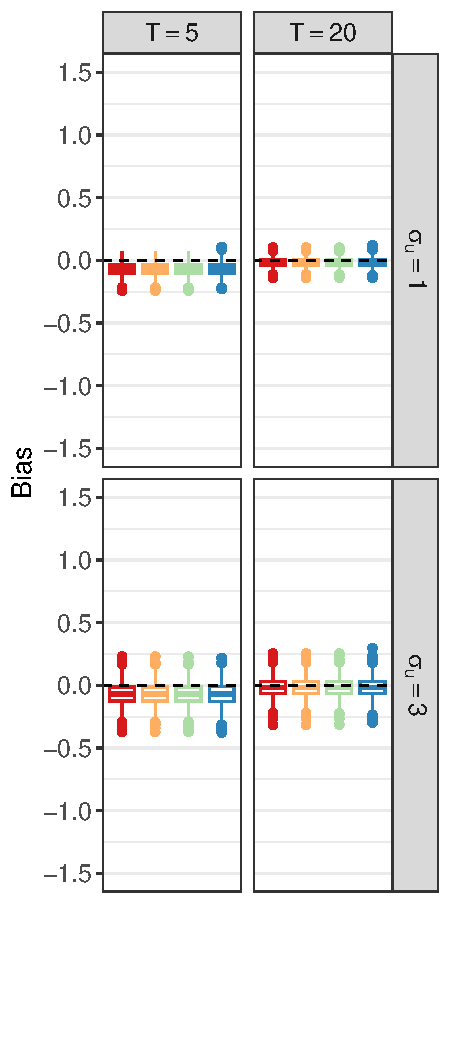
\includegraphics[height=10.6cm, keepaspectratio]{Figures/pred_continuous_out_continuous_bias_plot_T_total-vs-sd.u0_contextual.pdf}
        \caption{Contextual Effect $\gamma_{01}$ (Method MuCo)}\label{fig:dgm1-contextual}
    \end{subfigure}
    \label{fig:dgm1}
    \begin{flushleft}
        \begin{figurenote}
        The boxplot shows bias based on 1000 replications for data-generating model 1, which includes a continuous predictor and outcome. The boxes represent the interquartile range (IQR) from the 25th to 75th percentiles, with the median indicated by the horizontal line inside. Whiskers extend to 1.5 times the IQR, and replications outside this range are plotted as dots. UC = uncentered, CWC = centered within clusters, MuCo = Mundlak contextual, GLMM = generalized linear mixed model, GEE = generalized estimating equations. $T$ represents the total number of time points, and $\sigma_u$ denotes the random intercept residual variance. Y-axis breaks represent large intervals relative to bias but are consistent across data-generating models. In panel (a), GEE-UC with an independence correlation structure falls outside the plotted range, with estimates tightly clustered around 2.7 across all four scenarios.

        % The boxplot shows bias based on 1000 replications for data-generating model 1, which includes a continuous predictor and outcome. The boxes represent the interquartile range from the 25th to 75th percentiles, with the median indicated by the horizontal line inside. Whiskers extend to 1.5 times the IQR, and replications outside this range are plotted as dots. UC refers to uncentered, CWC to centered within clusters, and MuCo to Mundlak contextual, GLMM to generalized linear mixed model, GEE to generalized estimating equations. $T$ represents the total number of time points, and $\sigma_u$ denotes the random intercept residual variance. Y-axis breaks represent large intervals relative to bias but were chosen to be consistent across data-generating models. In panel (a), GEE-UC with independence correlation structure falls outside the plotted range, with estimates clustered tightly around 2.7 across all four scenarios.
        
        % Bias is shown for for data-generating model 1, which includes a continuous predictor and outcome. UC = uncentered; CWC = centered within clusters; MuCo = Mundlak contextual; $T$ = total number of time points; $\sigma_u$ = random intercept variance. Y-axis breaks represent large intervals relative to bias but were chosen to be consistent across data-generating models. In panel (a), GEE-UC with independence correlation structure falls outside the plotted range, with estimates clustered tightly around 2.7 across all four scenarios.
        
        % UC: Uncentered, CWC: centered within clusters, MuCo: Mundlak Contextual, T: total number of timepoints, $\sigma_u$: the random intercept residual variance. The breaks on the $Y$-axis represent large steps relative to bias, but were chosen to be consistent with the other DGMs. For panel (a), GEE-UC-independence fell outside the bounds, but has estimates tightly clustered around 2.7 (for all four scenarios).
    \end{figurenote}
    \end{flushleft}
\end{center}

% \begin{center}
%     \captionof{figure}{Bias for DGM 1 in Within-Person and Contextual Effect for Different Estimation Approaches}
%     \begin{subfigure}{1.1\linewidth}
%         \centering
%         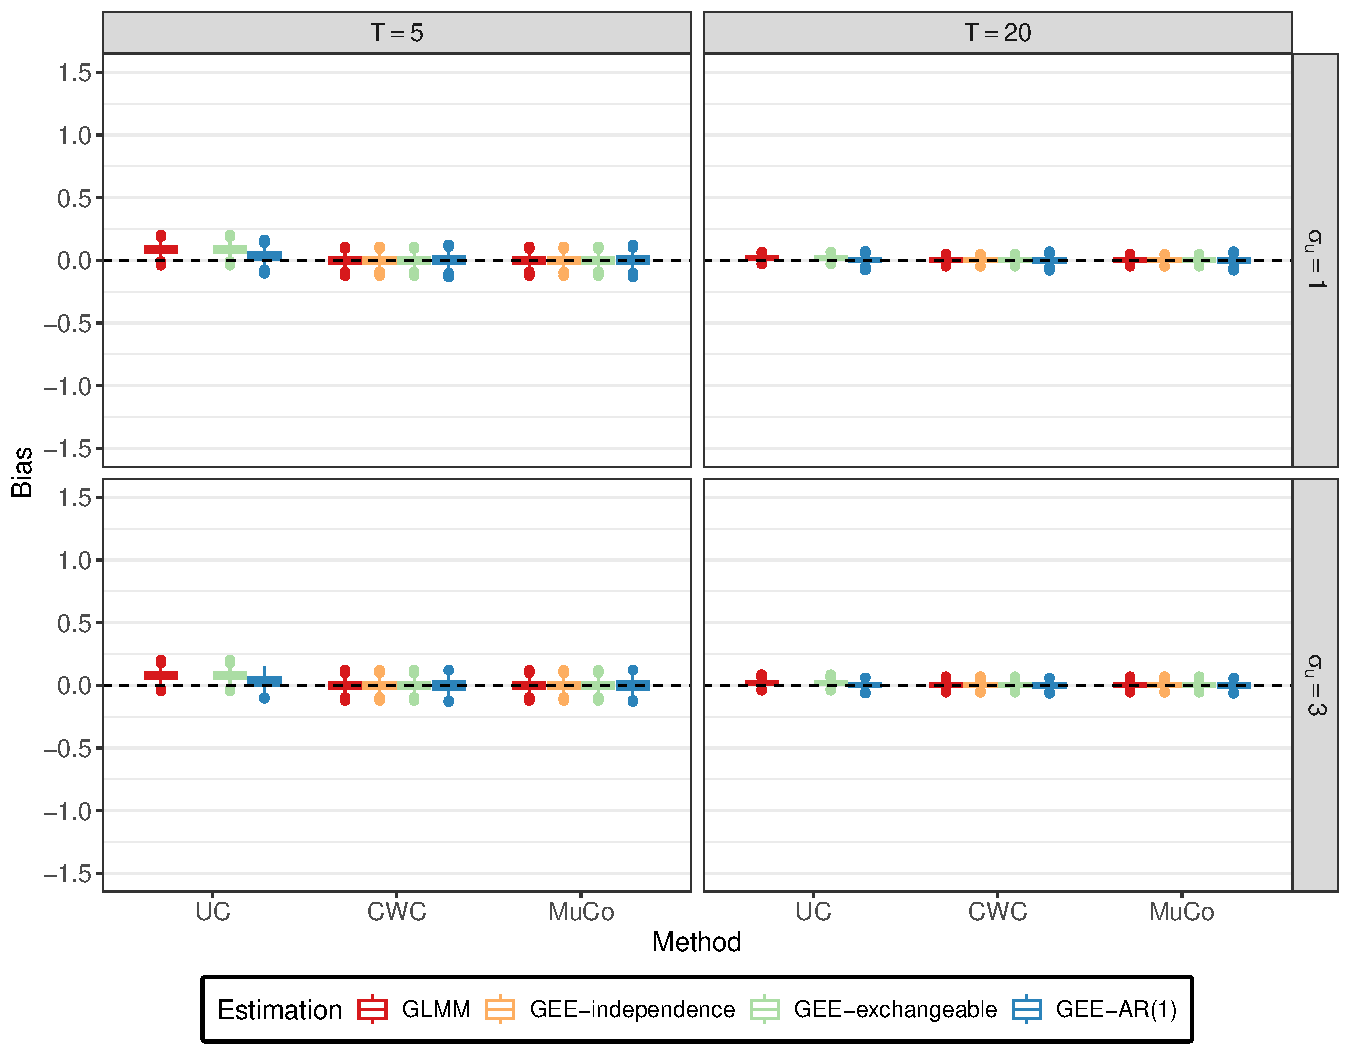
\includegraphics[width=\linewidth, keepaspectratio]{Figures/pred_continuous_out_continuous_bias_plot_T_total-vs-sd.u0_within.pdf}
%         \caption{Within-Person Effect}\label{fig:dgm1-within}
%     \end{subfigure}
%     \begin{subfigure}{1.1\linewidth}
%         \centering
%         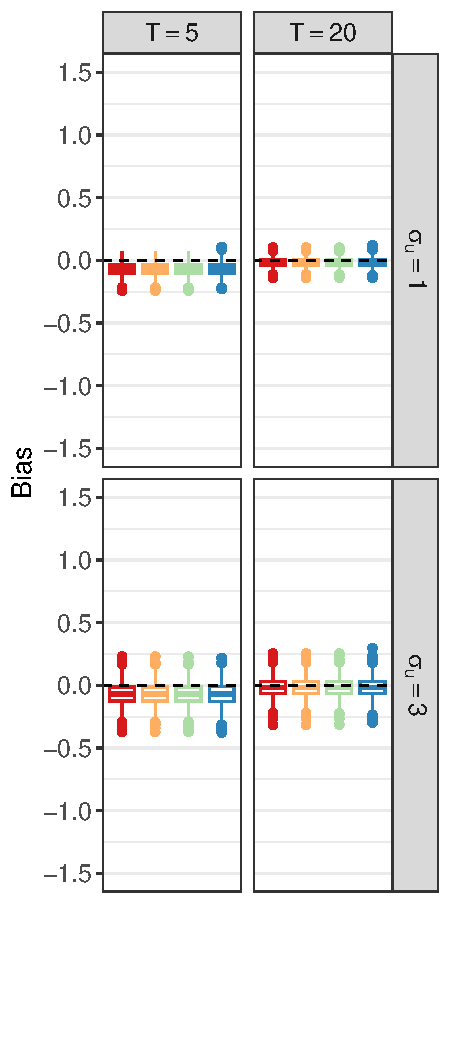
\includegraphics[width=\linewidth, keepaspectratio]{Figures/pred_continuous_out_continuous_bias_plot_T_total-vs-sd.u0_contextual.pdf}
%         \caption{Contextual Effect (Method 3)}\label{fig:dgm1-contextual}
%     \end{subfigure}
%     \label{fig:dgm1}
%     % \begin{figurenote}
%     %     \ldots
%     % \end{figurenote}
% \end{center}